En esta seccion vamos a realizar una conclusi\'on general de los distintos algoritmos. En base a la performance de los mismos y las distancias con respecto a la soluci\'on Exacta.

Primero planteamos un experimento en el cual corrimos para instancias aleatoreas, nuevamente con las tres densidades utilizadas a lo largo de todo el Trabajo Pr\'actico(15\%, 50\% y 100\%), todos los algoritmos (Exacto con podas, Heuristica Golosa, Heuristica de Busqueda Local y Heuristica GRASP con 5, 15 y 40 oteracioens respectivamente) unas 50 veces para cada cantidad de nodos entre 5 y 20 (por ser numeros manejables para el algoritmo exacto) para sacar un promedio de cuanto difiere cada Heuristica contra el algoritmo Exacto.\\
Para esto calculamos la peor soluci\'on para cada instancia (que ser\'ia ubicar todos los nodos en una \'unica partici\'on, con lo cual la sumatoria de las aristas intrapartici\'on ser\'a la sumatoria total de las aristas) y generamos una formula que nos representa un valor entre 1 y 0 que tanto diverge la Heuristica en relaci\'on al exacto, pero considerando el valor entre la peor soluci\'on y la soluci\'on ideal.
La formula es: 

\bc
1 - ((solucionHeuristica - solucionExacto)/(peorSolucion - solucionExacto))
\ec

Si la Heuristica tiene el mismo valor que el Exacto esta relaci\'on nos devuelve que es 1. Todo lo contrario si la heuristica devuelve la peor soluci\'on, esta formula nos retorna 0.\\
Con lo cual es un buen indicador para saber cuan buena es la soluci\'on de una de las heuristicas.

\subsection{Divergencia de las Heuristicas}

\subsubsection{2 Particiones}

\begin{figure}[H]
\begin{center}
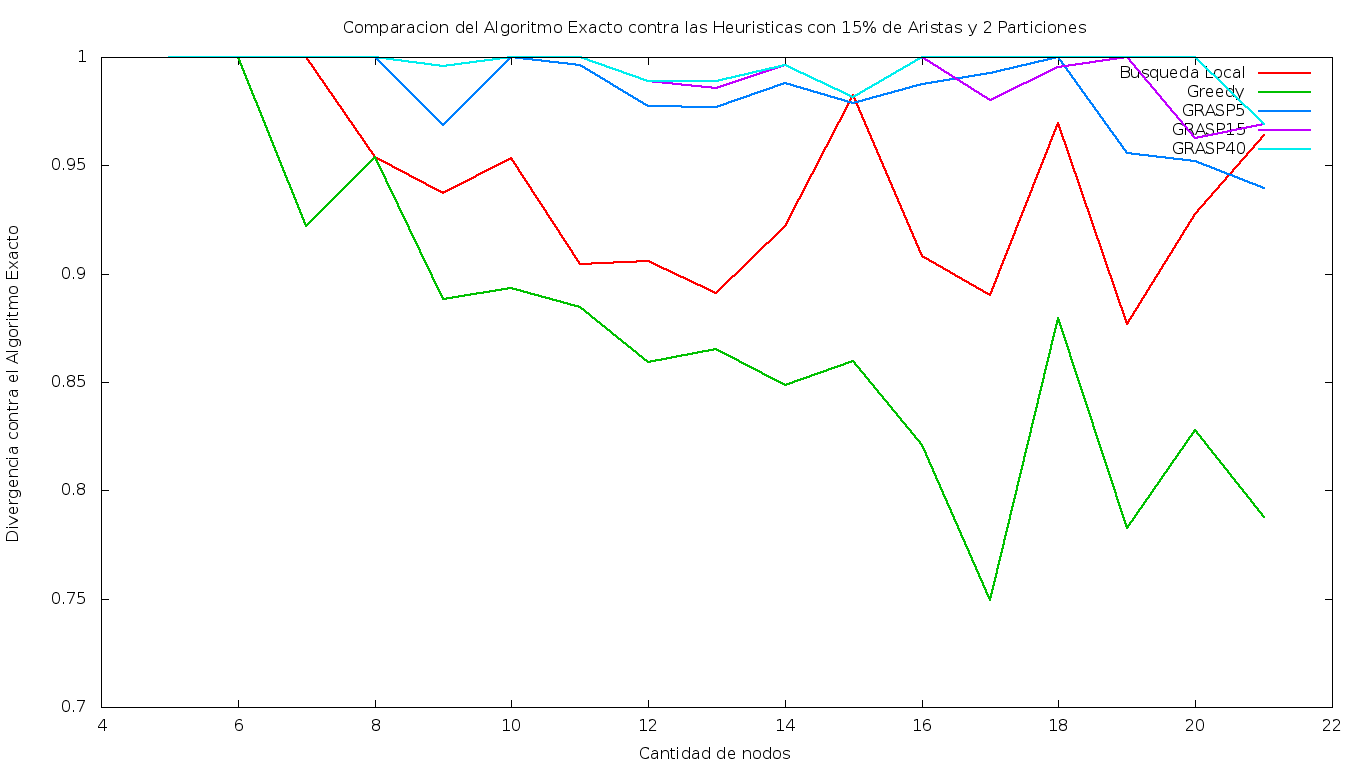
\includegraphics[scale=0.3]{finales/ComparacionesCon2Particiones15Aristas.png}
\caption{Distancias de las Heuristicas para K = 2 y 15\% de aristas}
\end{center}
\end{figure}

\begin{figure}[H]
\begin{center}
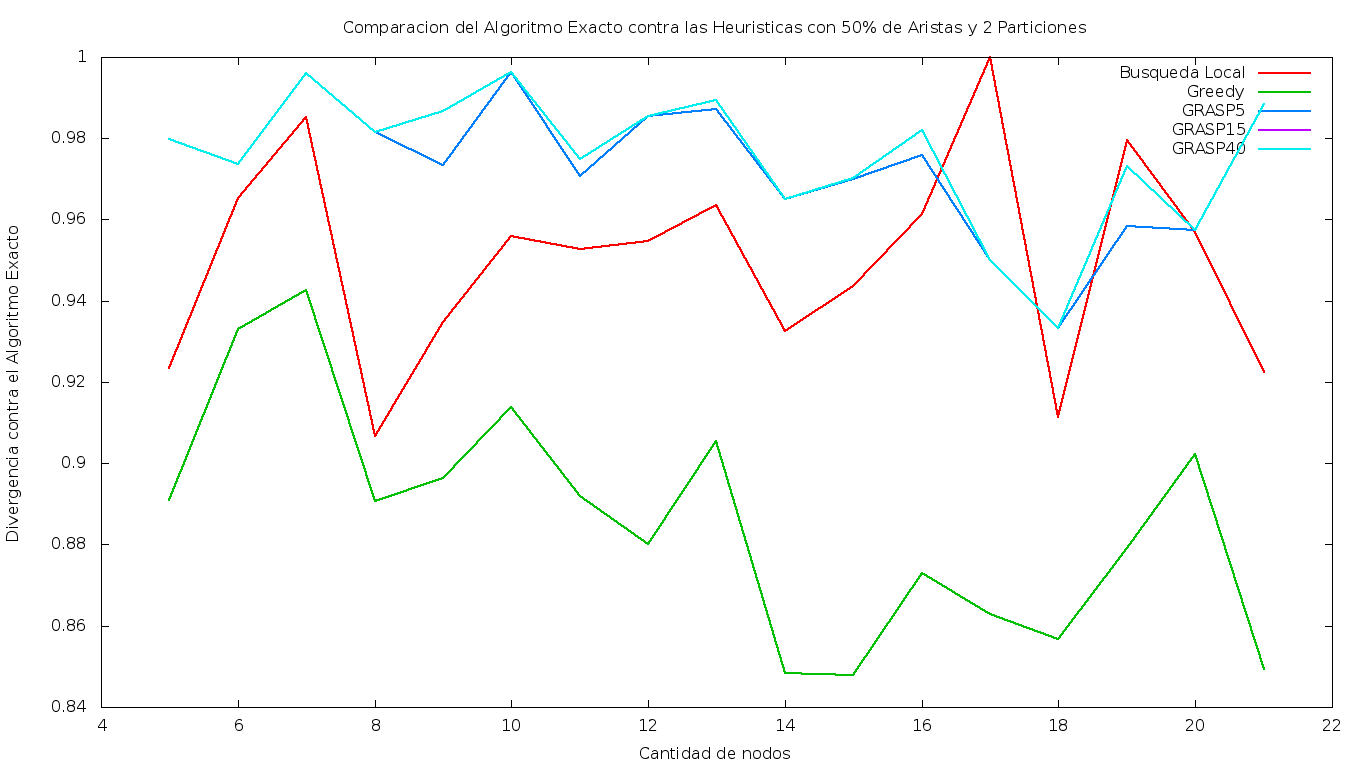
\includegraphics[scale=0.3]{finales/ComparacionesCon2Particiones50Aristas.png}
\caption{Distancias de las Heuristicas para K = 2 y 50\% de aristas}
\end{center}
\end{figure}

\begin{figure}[H]
\begin{center}
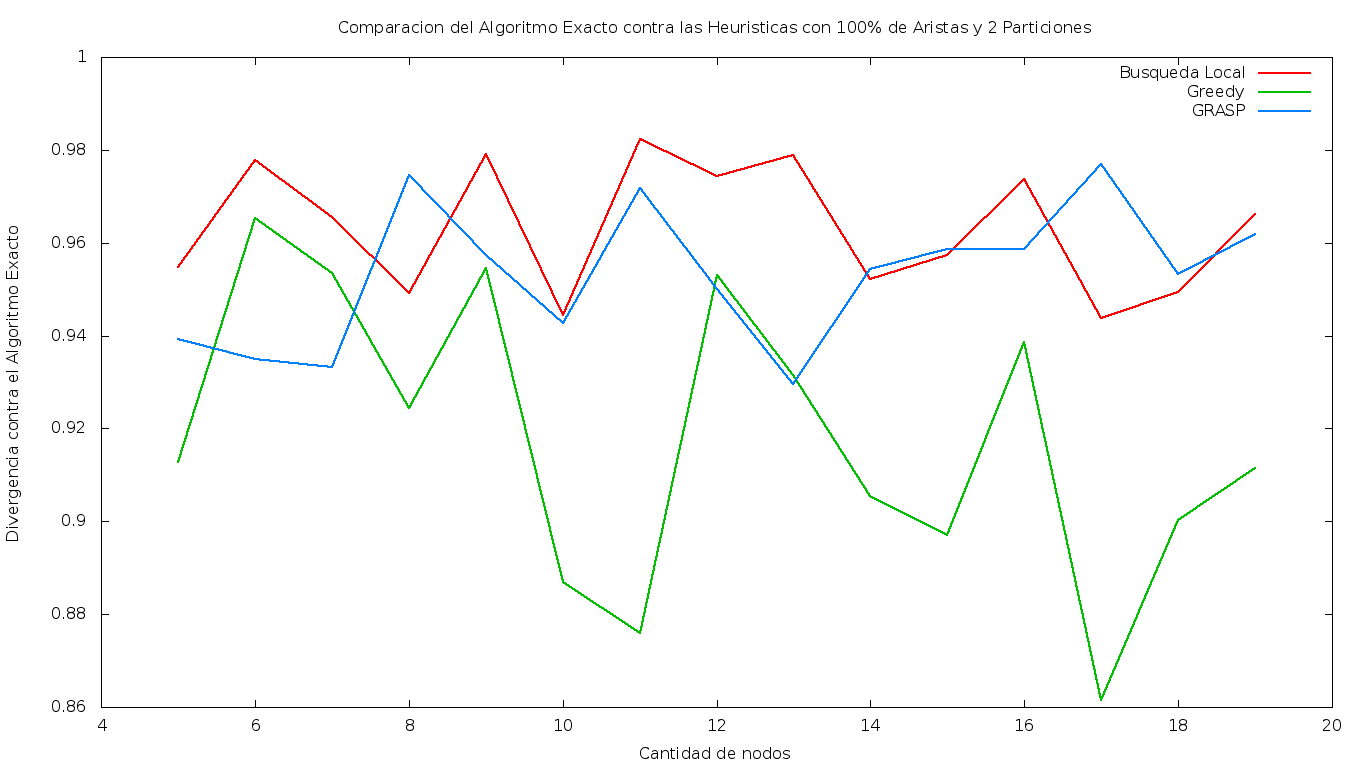
\includegraphics[scale=0.3]{finales/ComparacionesCon2Particiones100Aristas.png}
\caption{Distancias de las Heuristicas para K = 2 y 100\% de aristas}
\end{center}
\end{figure}

\subsubsection{3 Particiones}

\begin{figure}[H]
\begin{center}
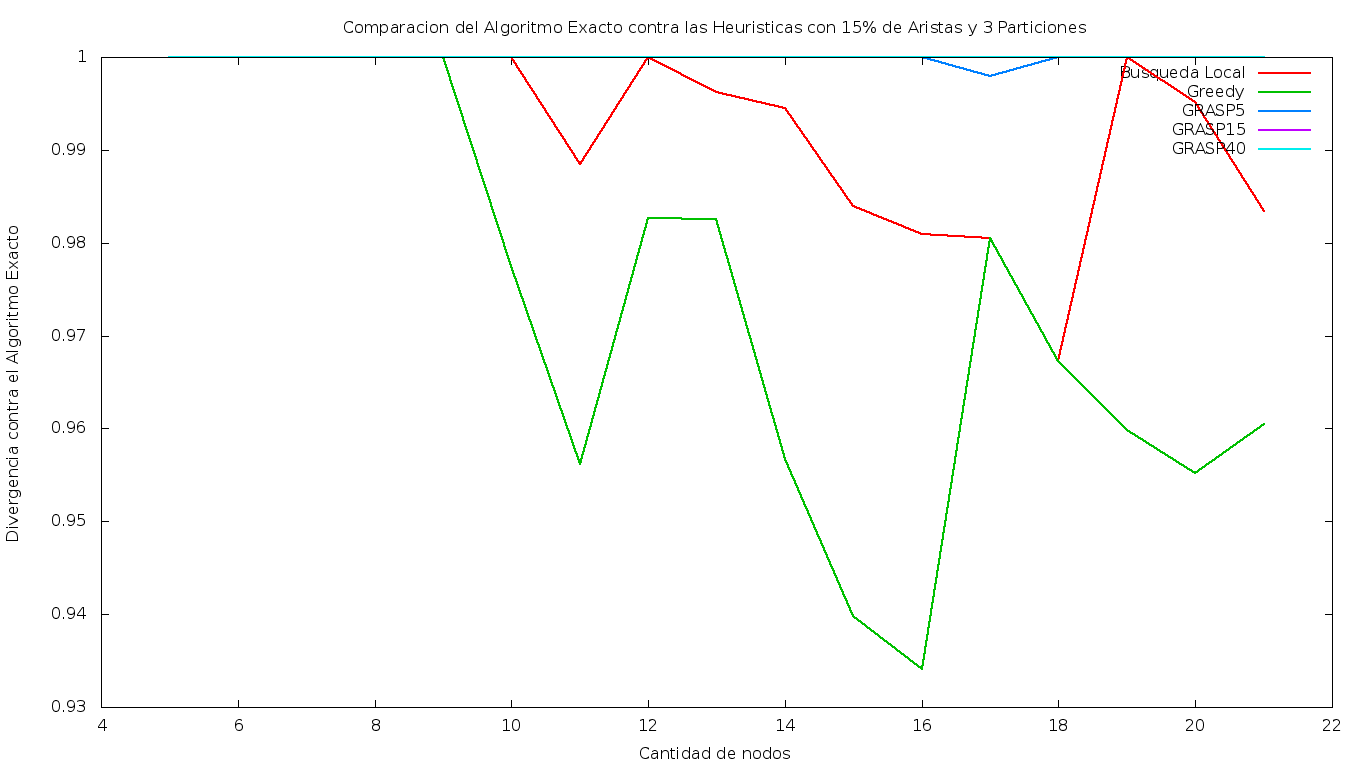
\includegraphics[scale=0.3]{finales/ComparacionesCon3Particiones15Aristas.png}
\caption{Distancias de las Heuristicas para K = 3 y 15\% de aristas}
\end{center}
\end{figure}

\begin{figure}[H]
\begin{center}
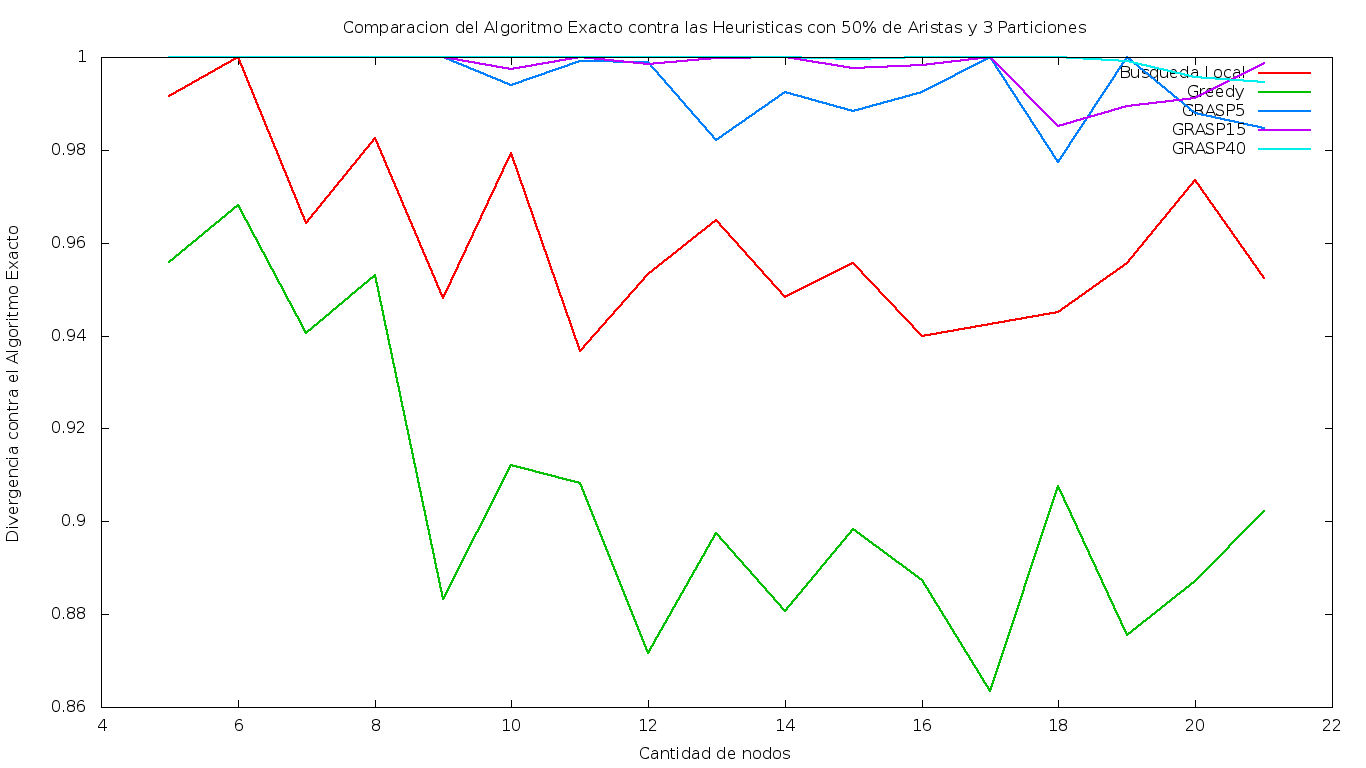
\includegraphics[scale=0.3]{finales/ComparacionesCon3Particiones50Aristas.png}
\caption{Distancias de las Heuristicas para K = 3 y 50\% de aristas}
\end{center}
\end{figure}

\begin{figure}[H]
\begin{center}
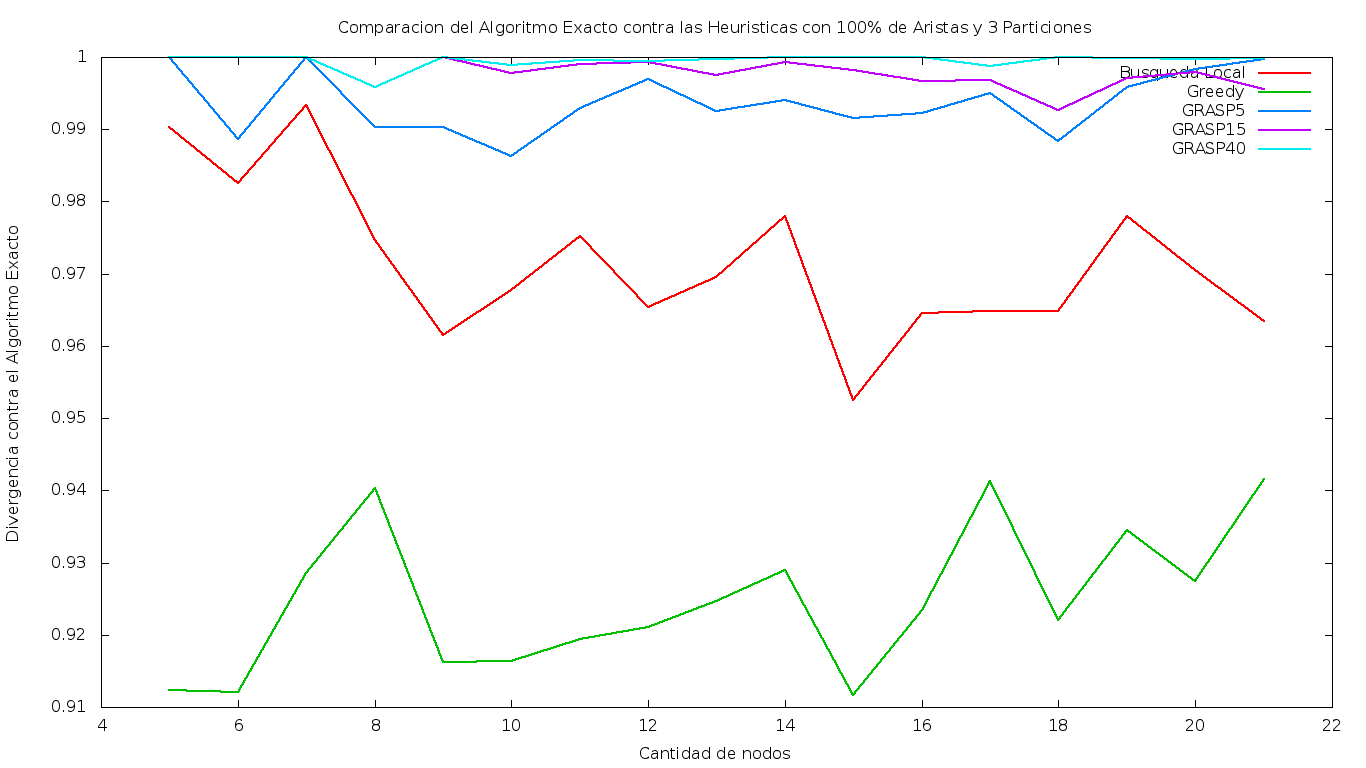
\includegraphics[scale=0.3]{finales/ComparacionesCon3Particiones100Aristas.png}
\caption{Distancias de las Heuristicas para K = 3 y 100\% de aristas}
\end{center}
\end{figure}


\subsubsection{4 Particiones}

\begin{figure}[H]
\begin{center}
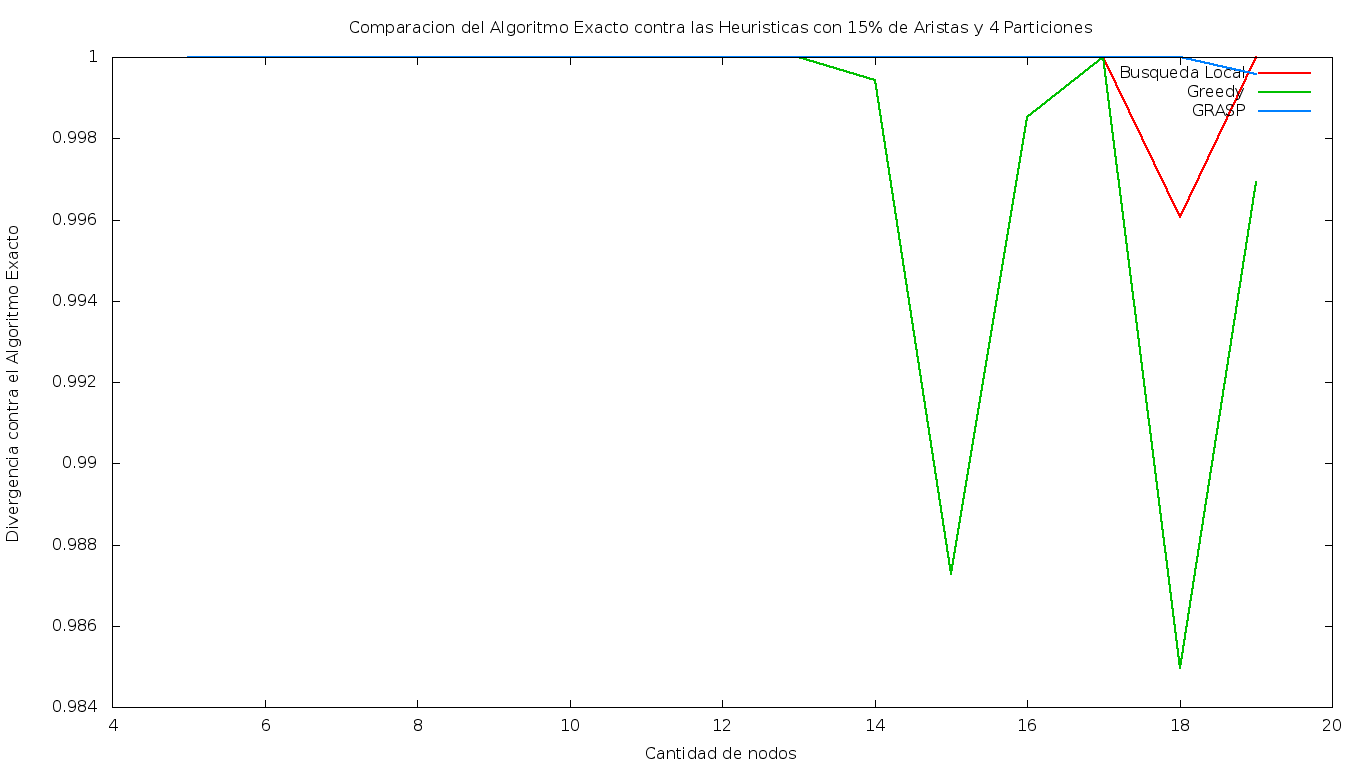
\includegraphics[scale=0.3]{finales/ComparacionesCon4Particiones15Aristas.png}
\caption{Distancias de las Heuristicas para K = 4 y 15\% de aristas}
\end{center}
\end{figure}

\begin{figure}[H]
\begin{center}
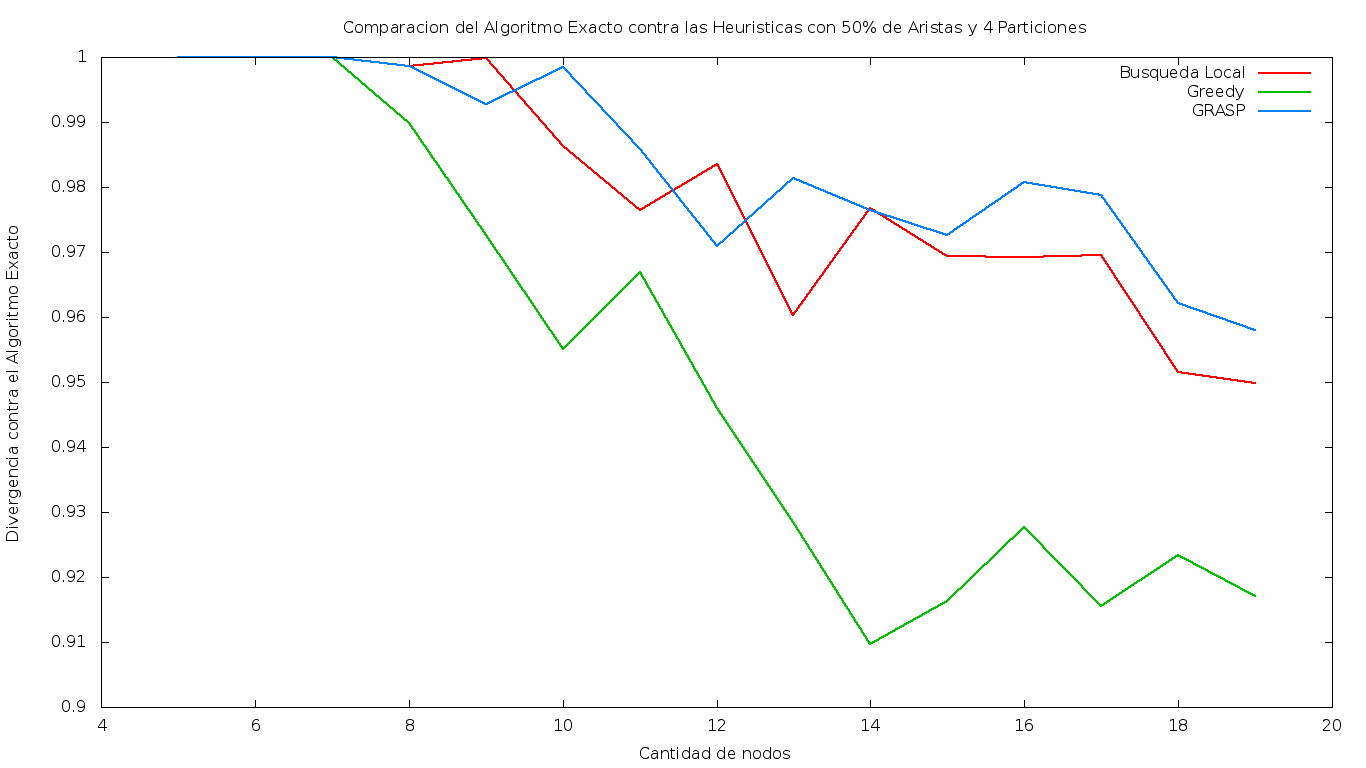
\includegraphics[scale=0.3]{finales/ComparacionesCon4Particiones50Aristas.png}
\caption{Distancias de las Heuristicas para K = 4 y 50\% de aristas}
\end{center}
\end{figure}

\begin{figure}[H]
\begin{center}
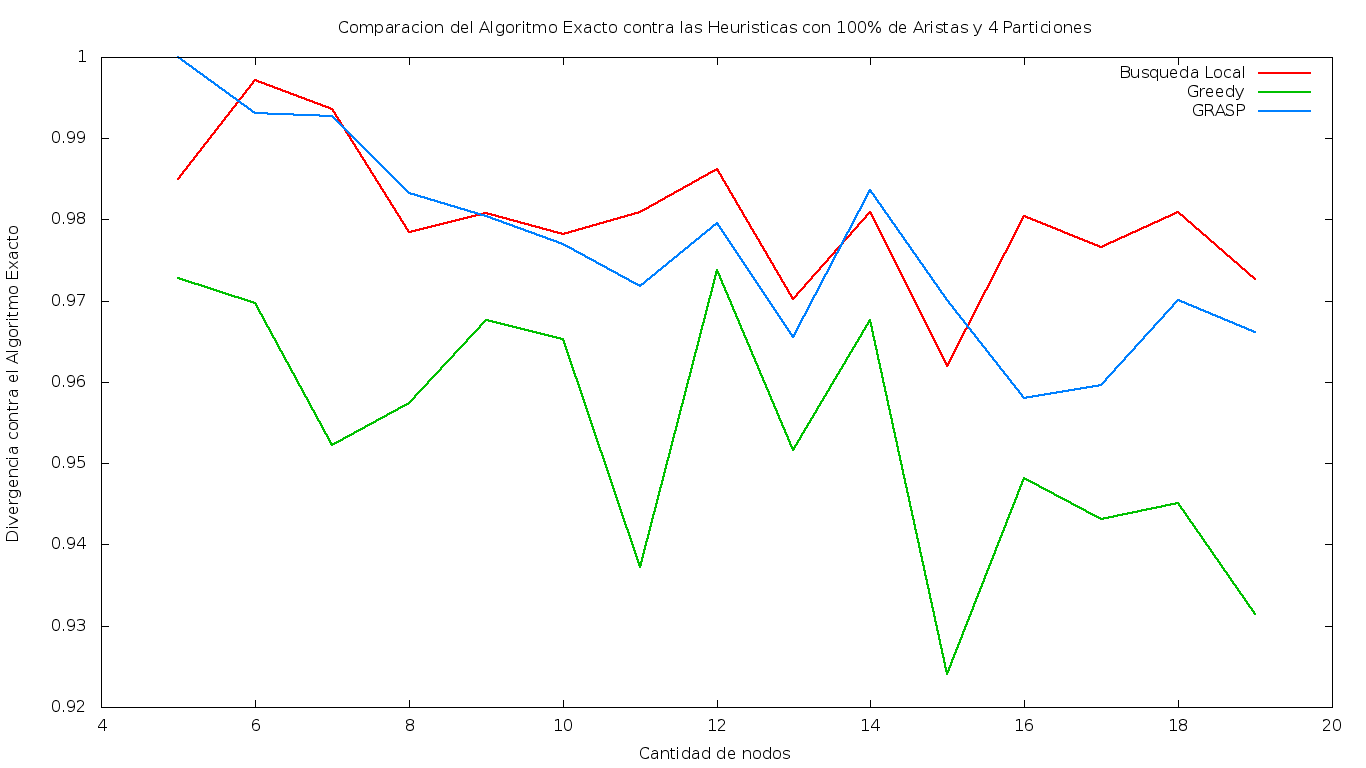
\includegraphics[scale=0.3]{finales/ComparacionesCon4Particiones100Aristas.png}
\caption{Distancias de las Heuristicas para K = 4 y 100\% de aristas}
\end{center}
\end{figure}

\subsubsection{5 Particiones}

\begin{figure}[H]
\begin{center}
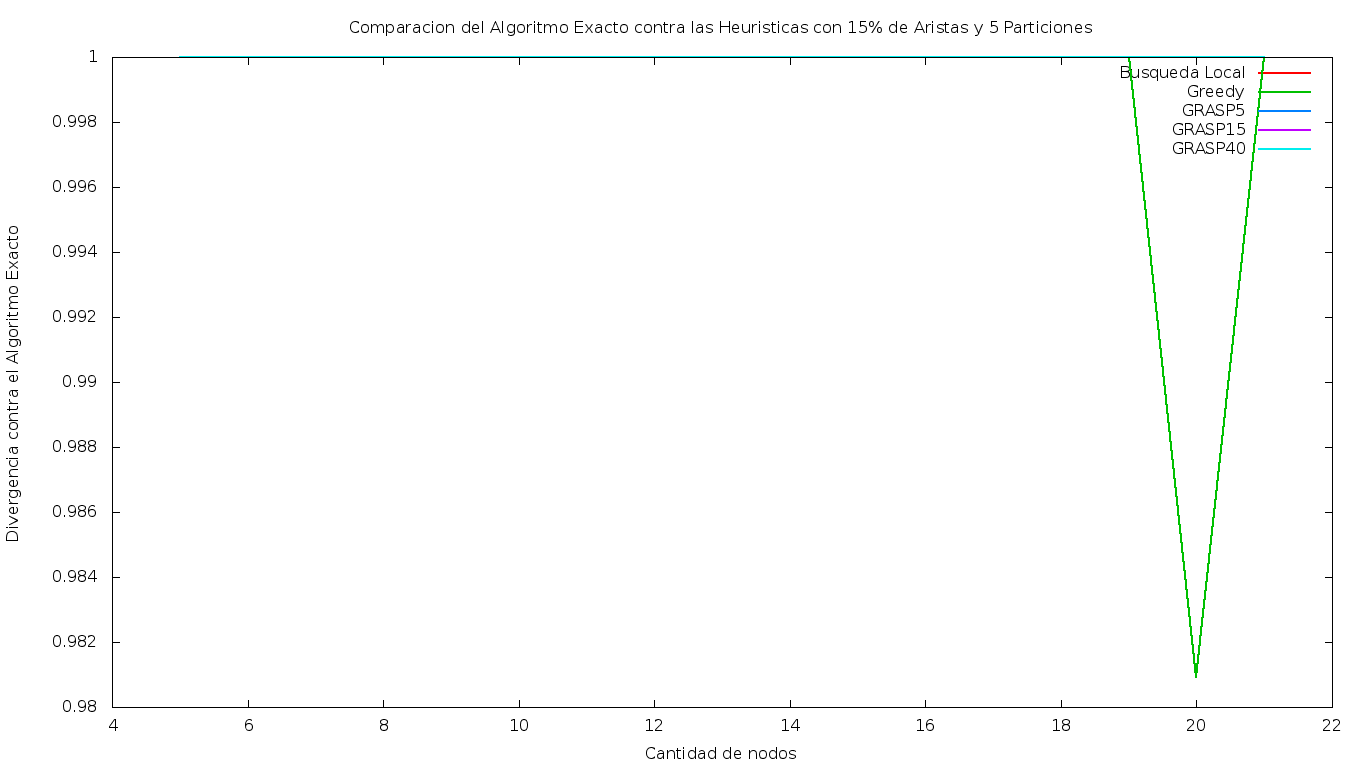
\includegraphics[scale=0.3]{finales/ComparacionesCon5Particiones15Aristas.png}
\caption{Distancias de las Heuristicas para K = 5 y 15\% de aristas}
\end{center}
\end{figure}

\begin{figure}[H]
\begin{center}
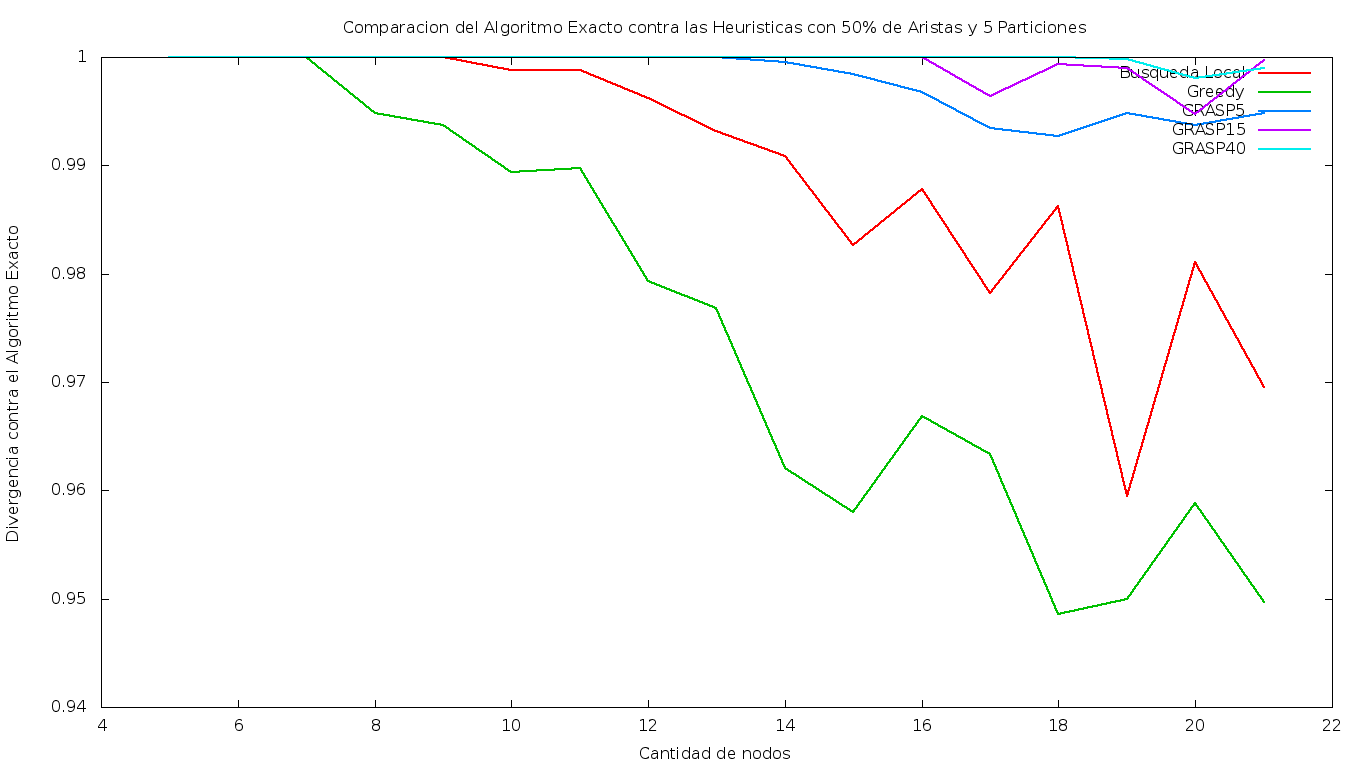
\includegraphics[scale=0.3]{finales/ComparacionesCon5Particiones50Aristas.png}
\caption{Distancias de las Heuristicas para K = 5 y 50\% de aristas}
\end{center}
\end{figure}

\begin{figure}[H]
\begin{center}
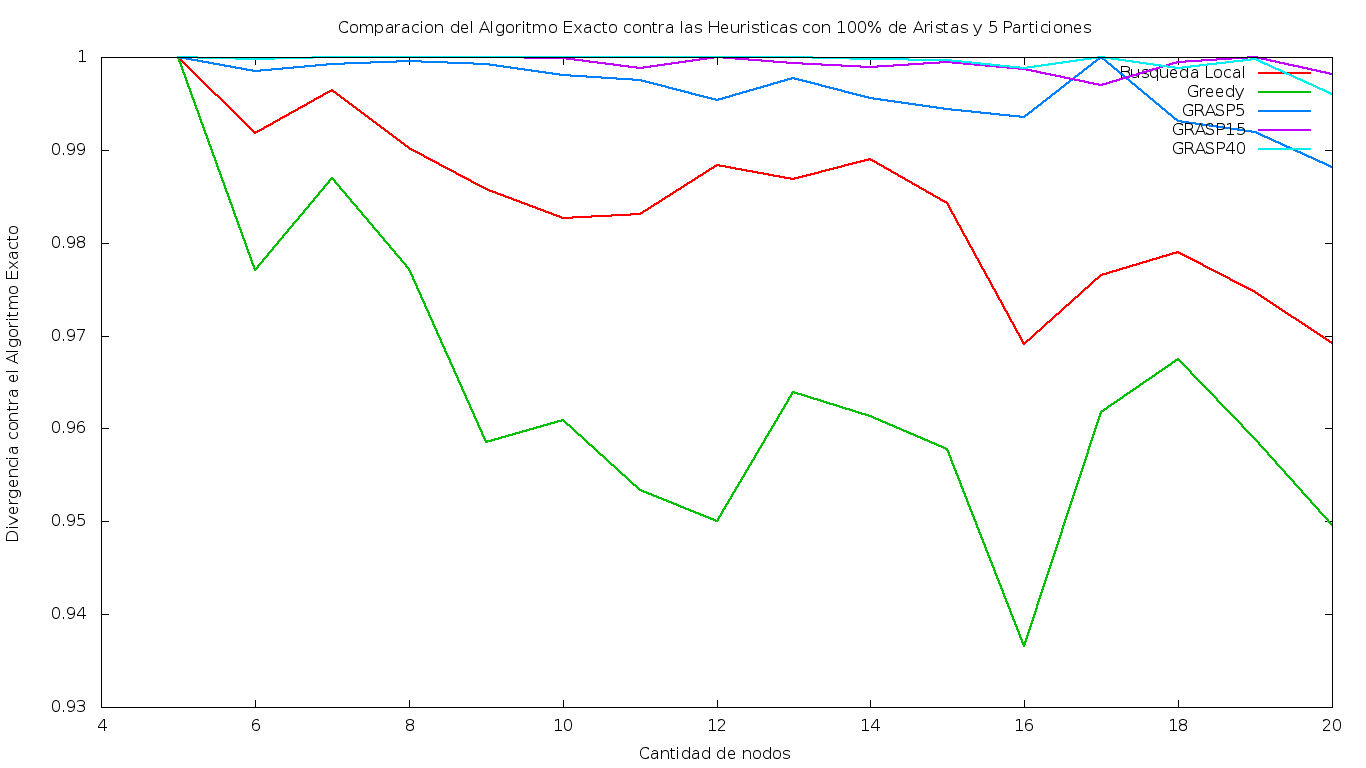
\includegraphics[scale=0.3]{finales/ComparacionesCon5Particiones100Aristas.png}
\caption{Distancias de las Heuristicas para K = 5 y 100\% de aristas}
\end{center}
\end{figure}

\subsubsection{6 Particiones}

\begin{figure}[H]
\begin{center}
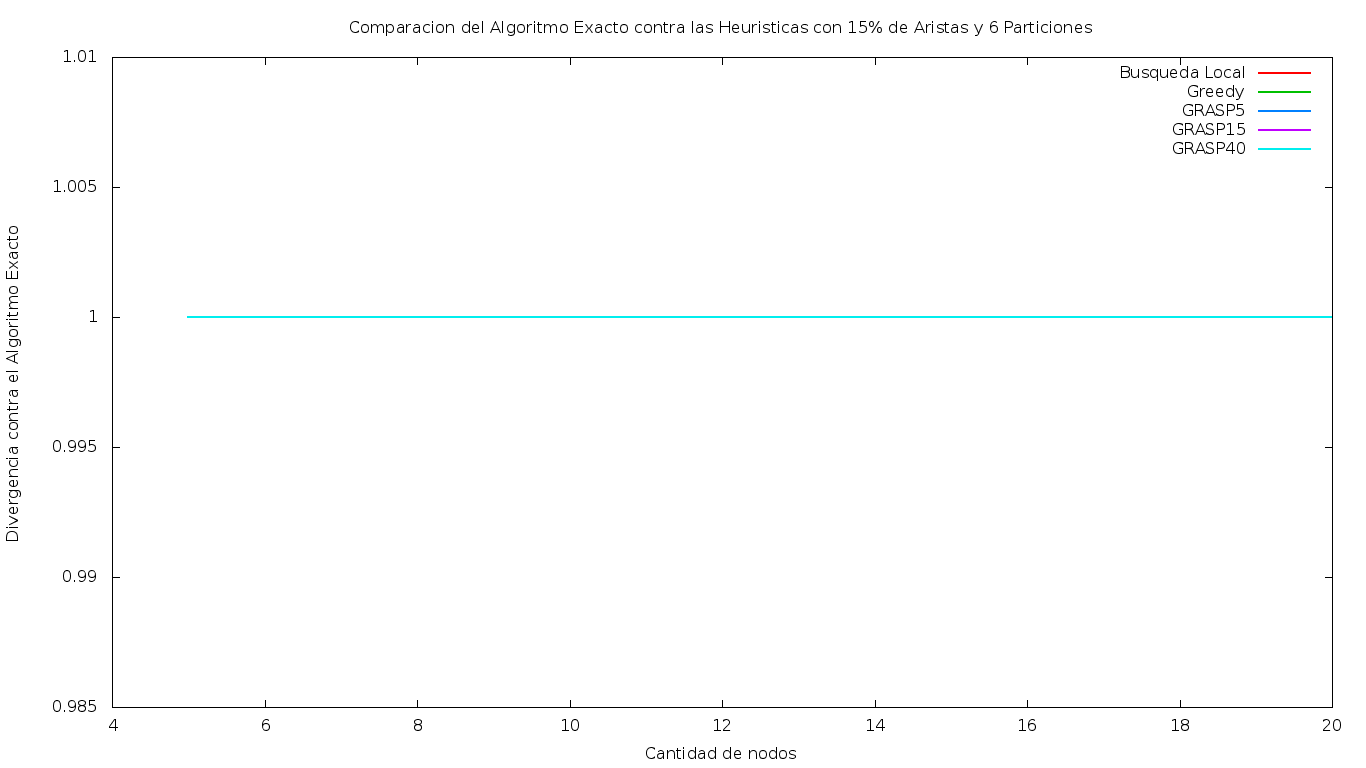
\includegraphics[scale=0.3]{finales/ComparacionesCon6Particiones15Aristas.png}
\caption{Distancias de las Heuristicas para K = 6 y 15\% de aristas}
\end{center}
\end{figure}

\begin{figure}[H]
\begin{center}
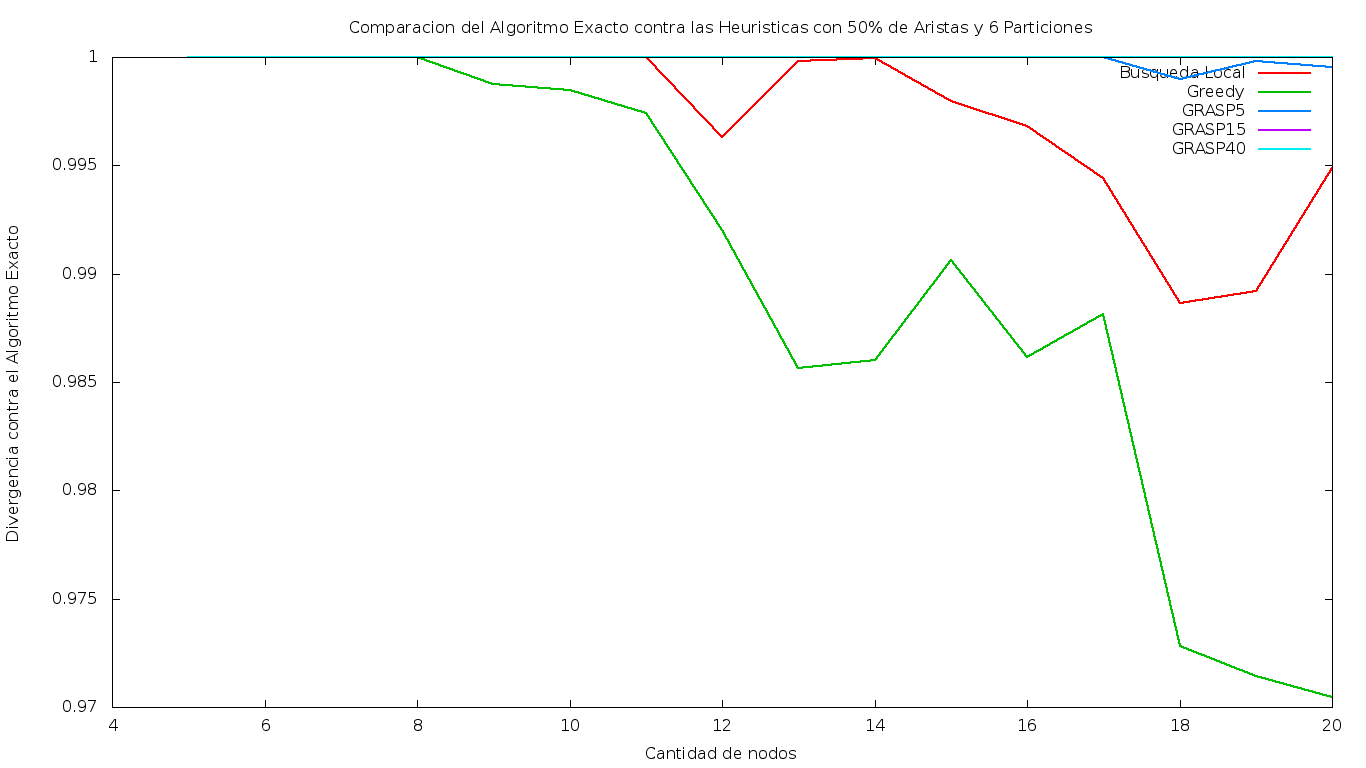
\includegraphics[scale=0.3]{finales/ComparacionesCon6Particiones50Aristas.png}
\caption{Distancias de las Heuristicas para K = 6 y 50\% de aristas}
\end{center}
\end{figure}

\begin{figure}[H]
\begin{center}
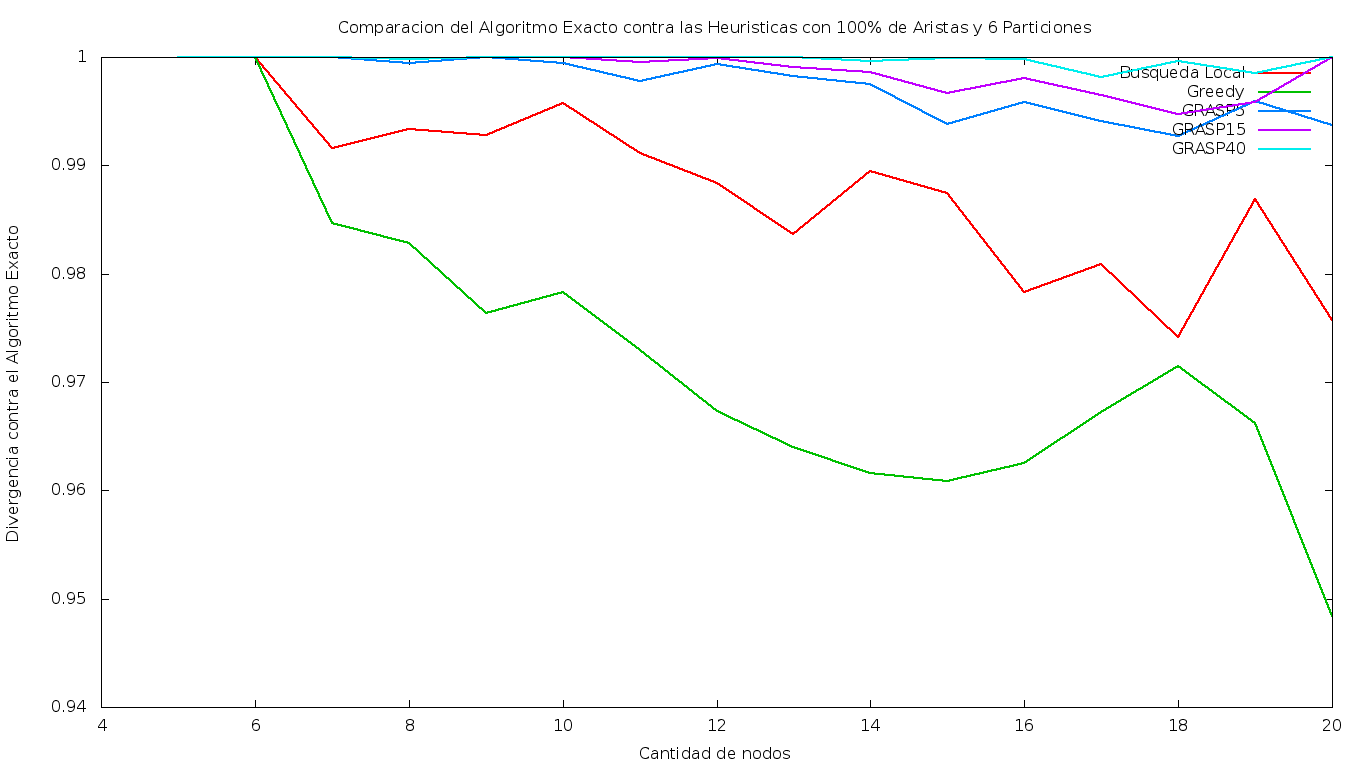
\includegraphics[scale=0.3]{finales/ComparacionesCon6Particiones100Aristas.png}
\caption{Distancias de las Heuristicas para K = 6 y 100\% de aristas}
\end{center}
\end{figure}

\subsubsection{7 Particiones}

\begin{figure}[H]
\begin{center}
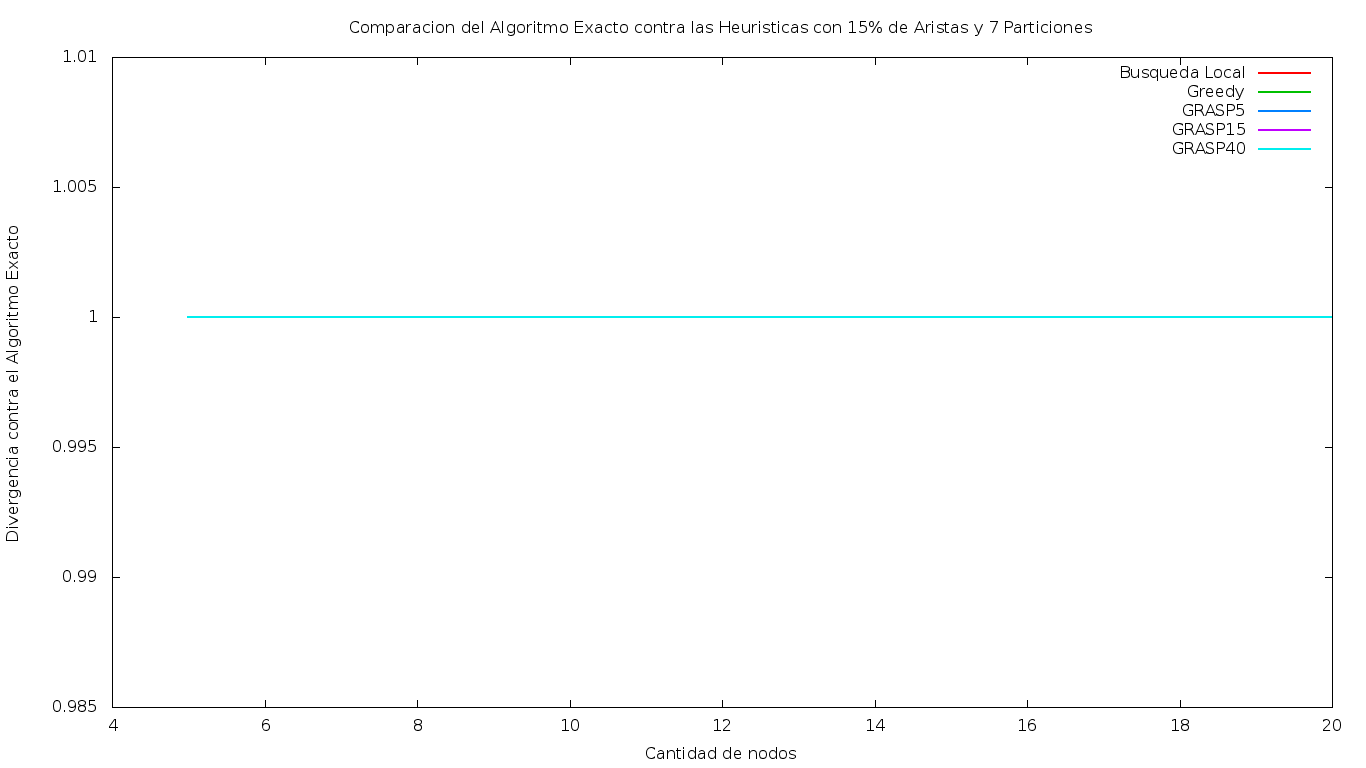
\includegraphics[scale=0.3]{finales/ComparacionesCon7Particiones15Aristas.png}
\caption{Distancias de las Heuristicas para K = 7 y 15\% de aristas}
\end{center}
\end{figure}

\begin{figure}[H]
\begin{center}
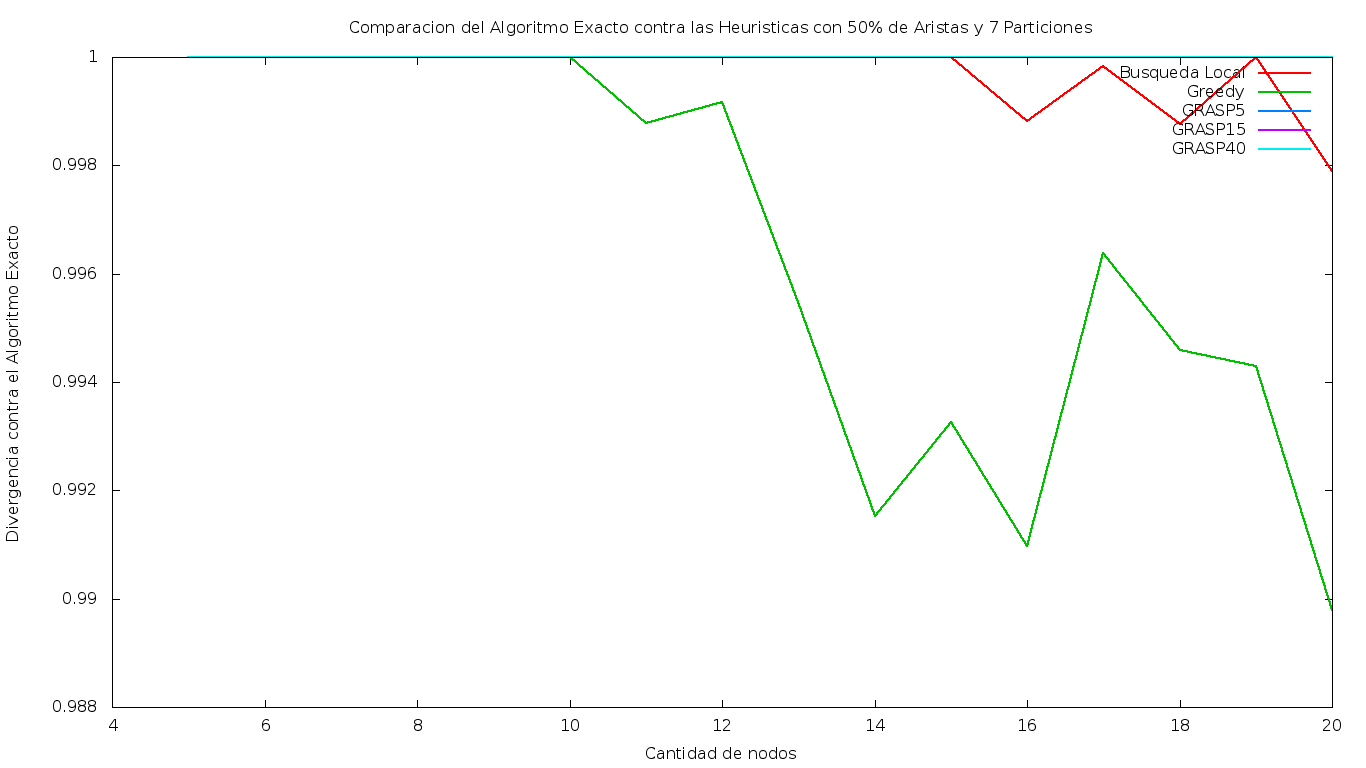
\includegraphics[scale=0.3]{finales/ComparacionesCon7Particiones50Aristas.png}
\caption{Distancias de las Heuristicas para K = 7 y 50\% de aristas}
\end{center}
\end{figure}

\begin{figure}[H]
\begin{center}
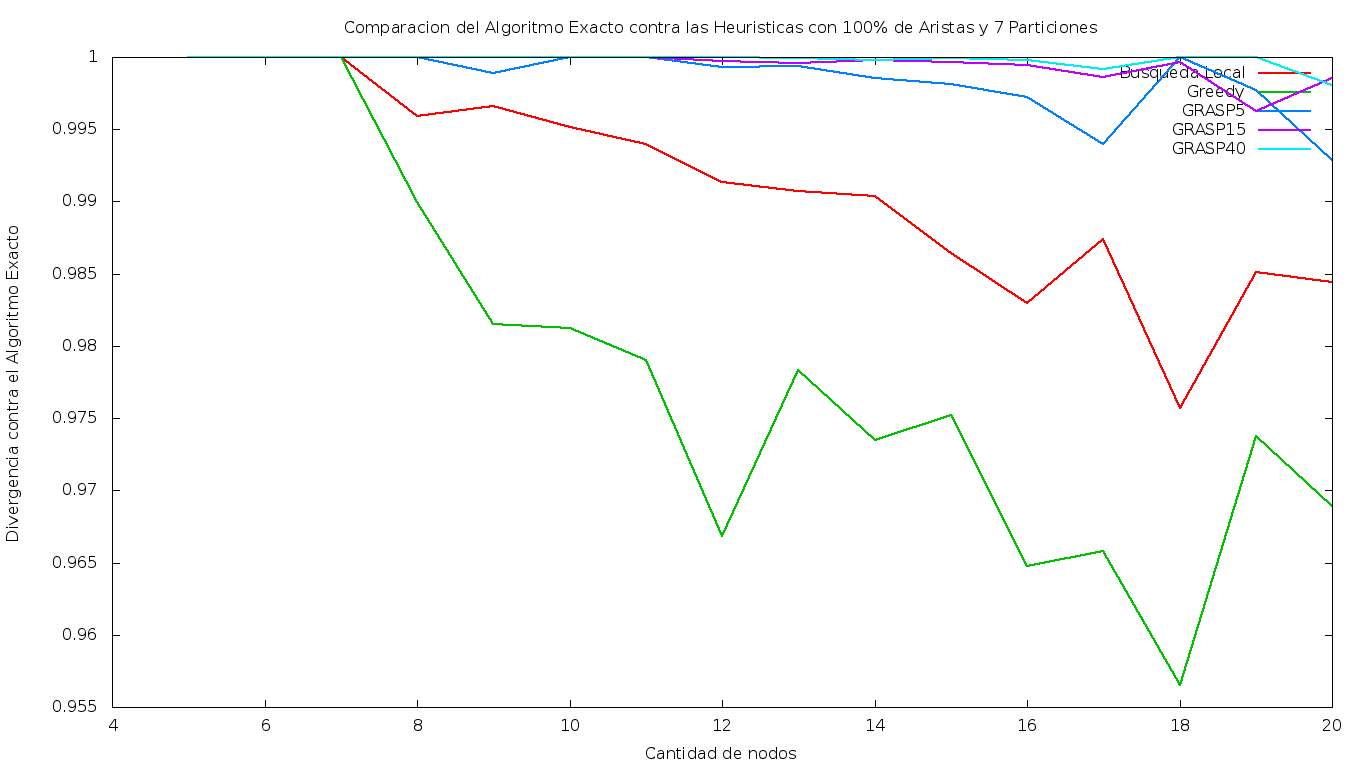
\includegraphics[scale=0.3]{finales/ComparacionesCon7Particiones100Aristas.png}
\caption{Distancias de las Heuristicas para K = 7 y 100\% de aristas}
\end{center}
\end{figure}



Podemos ver como a medida que aumenta la cantida de nodos los valores de divergencia de las Heur\'isticas comienzan a aumentar.\\

Otro punto f\'acilmente apreciable es que la Heur\'istica Greedy es la que mayor distancia tiene con respecto a la soluci\'on Exacta para todos los valores de n y cantidad de particiones, seguida por Busqueda Local y luego como, es de esperarse, los GRASP con distinta cantidad de iteraciones.\\

Volvemos a ver como al aumentar la cantidad de particiones, en funcion de las densidades del grafo, para grafos menos densos, en todos los algoritmos las soluciones se acercan mucho mas a la Ecxacta. Como ya lo mencionamos en alg\'un momento esto debe ser produco de la libertad que tengo de colocar los nodos al tener un grafo poco denso (que probablemnte tanga una gran cantidad de nodos aislados y una menor aristas intrapartici\'ones).

No podemos apreciar bien los valores de los distintos GRASP con sus respectiva cantidad de repeticiones, ya que para estas cantidades de nodos y particiones todos devuelven resultados muy similares.\\
Por este motivo vamos a realizar m\'as experimentos pero excuptuando al algoritmo exacto para poder correr instancias m\'as grandes.


\section{Divergencia para instancias mayores}

Usamos el mismo cr\'iterio de comparacion que en el ejercicio anterior. Pero en vez de utilizar el excato como patr\'on utilizamos el GRASP con 40 repeticiones. Los valores para la cantidad de particiones seleccionados fueron 5, 30 y 100

\subsubsection{5 Particiones}

\begin{figure}[H]
\begin{center}
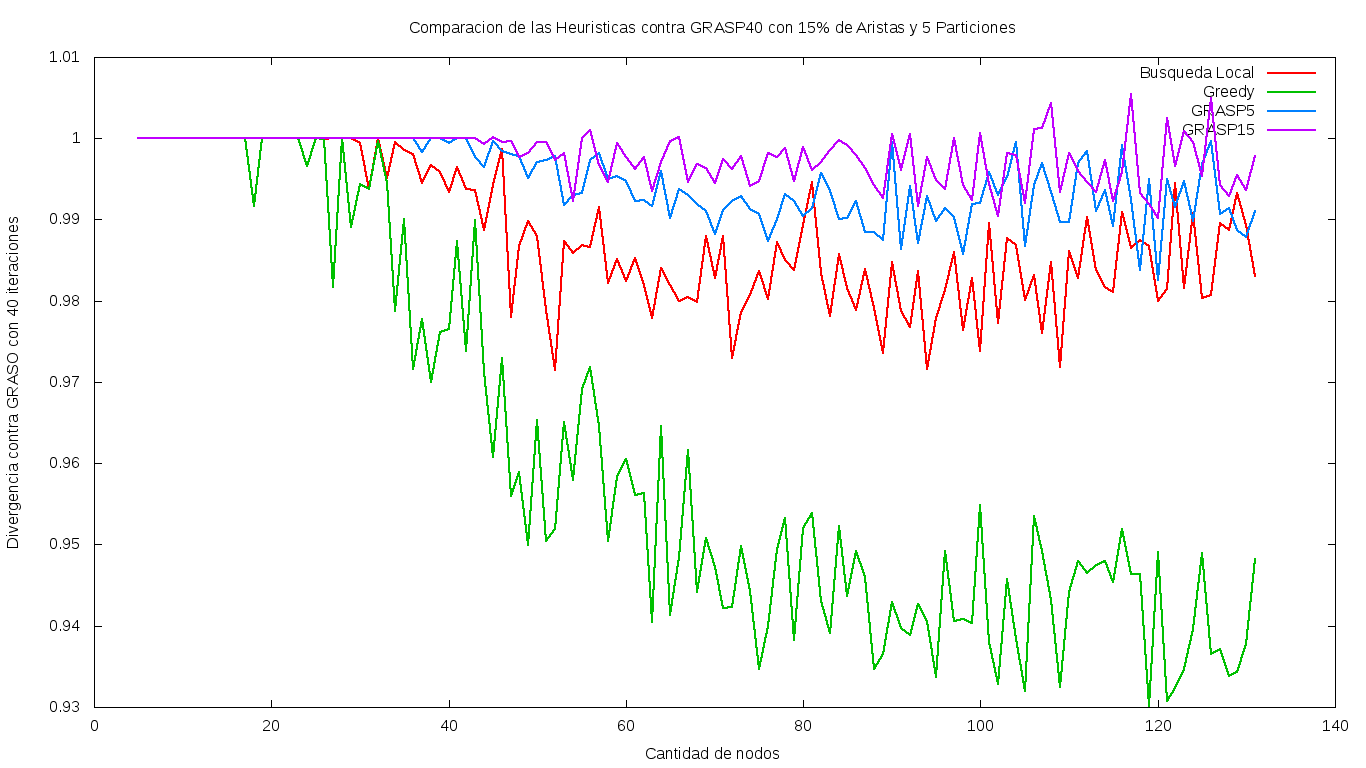
\includegraphics[scale=0.4]{finales/muchosComparacionesCon5Particiones15Aristas.png}
\caption{Distancias de las soluciones para K = 5 y 15\% de aristas}
\end{center}
\end{figure}

\begin{figure}[H]
\begin{center}
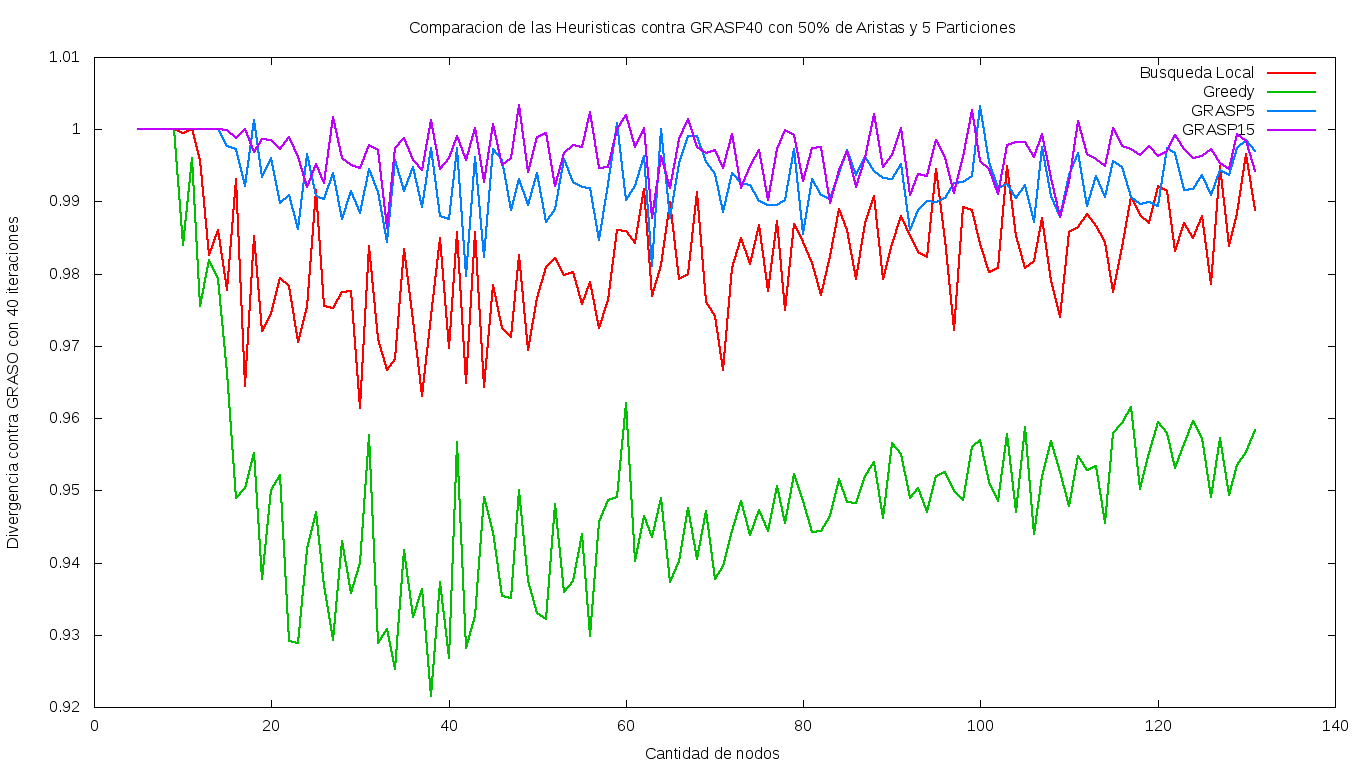
\includegraphics[scale=0.4]{finales/muchosComparacionesCon5Particiones50Aristas.png}
\caption{Distancias de las solucioens para K = 5 y 50\% de aristas}
\end{center}
\end{figure}

\begin{figure}[H]
\begin{center}
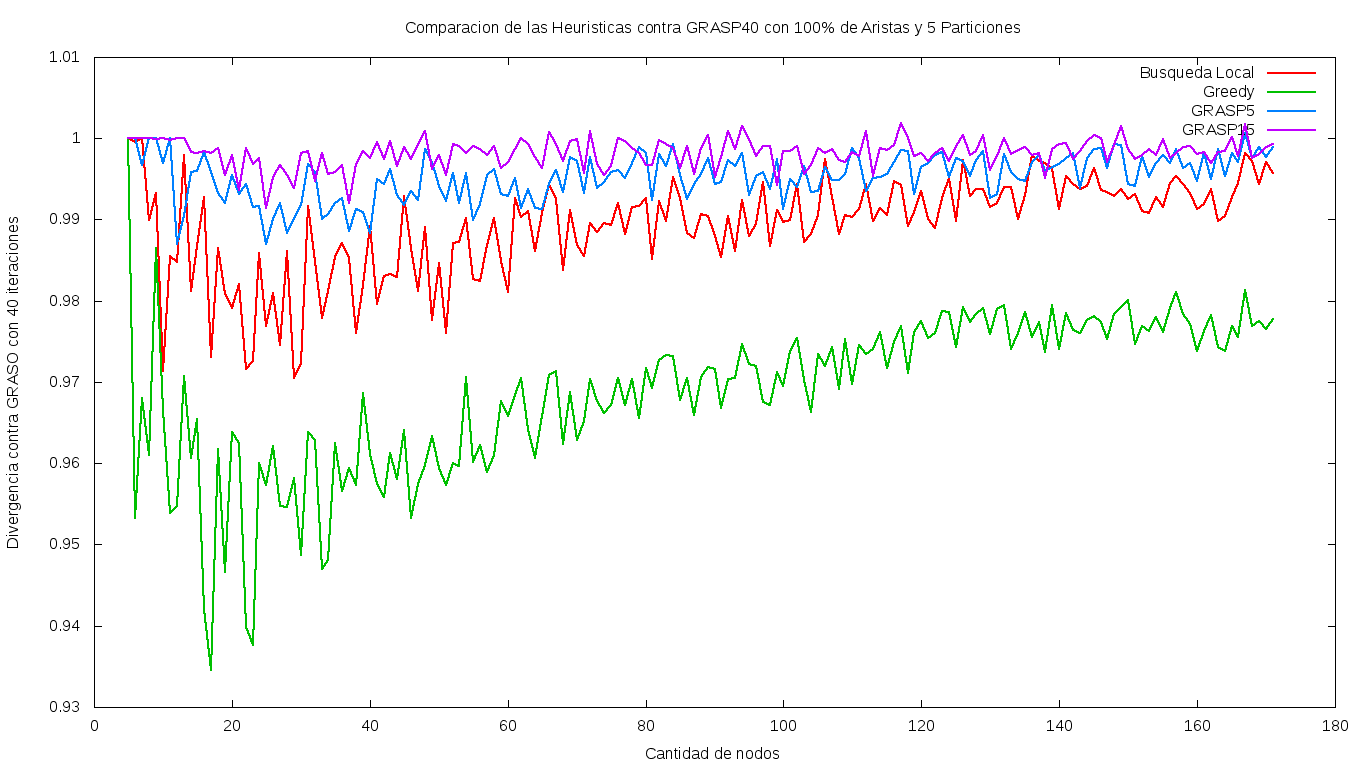
\includegraphics[scale=0.4]{finales/muchosComparacionesCon5Particiones100Aristas.png}
\caption{Distancias de las solucioens para K = 5 y 100\% de aristas}
\end{center}
\end{figure}

\subsubsection{30 Particiones}

\begin{figure}[H]
\begin{center}
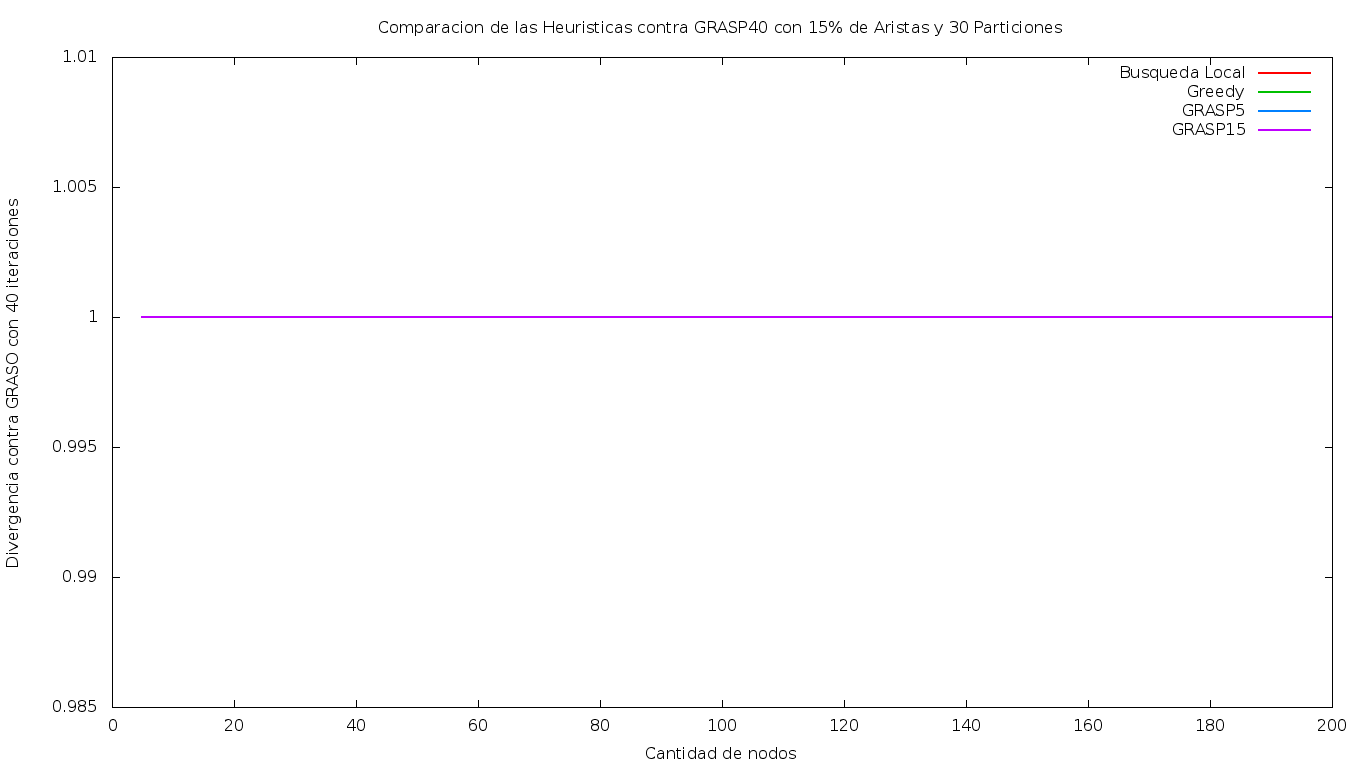
\includegraphics[scale=0.4]{finales/muchosComparacionesCon30Particiones15Aristas.png}
\caption{Distancias de las soluciones para K = 30 y 15\% de aristas}
\end{center}
\end{figure}

\begin{figure}[H]
\begin{center}
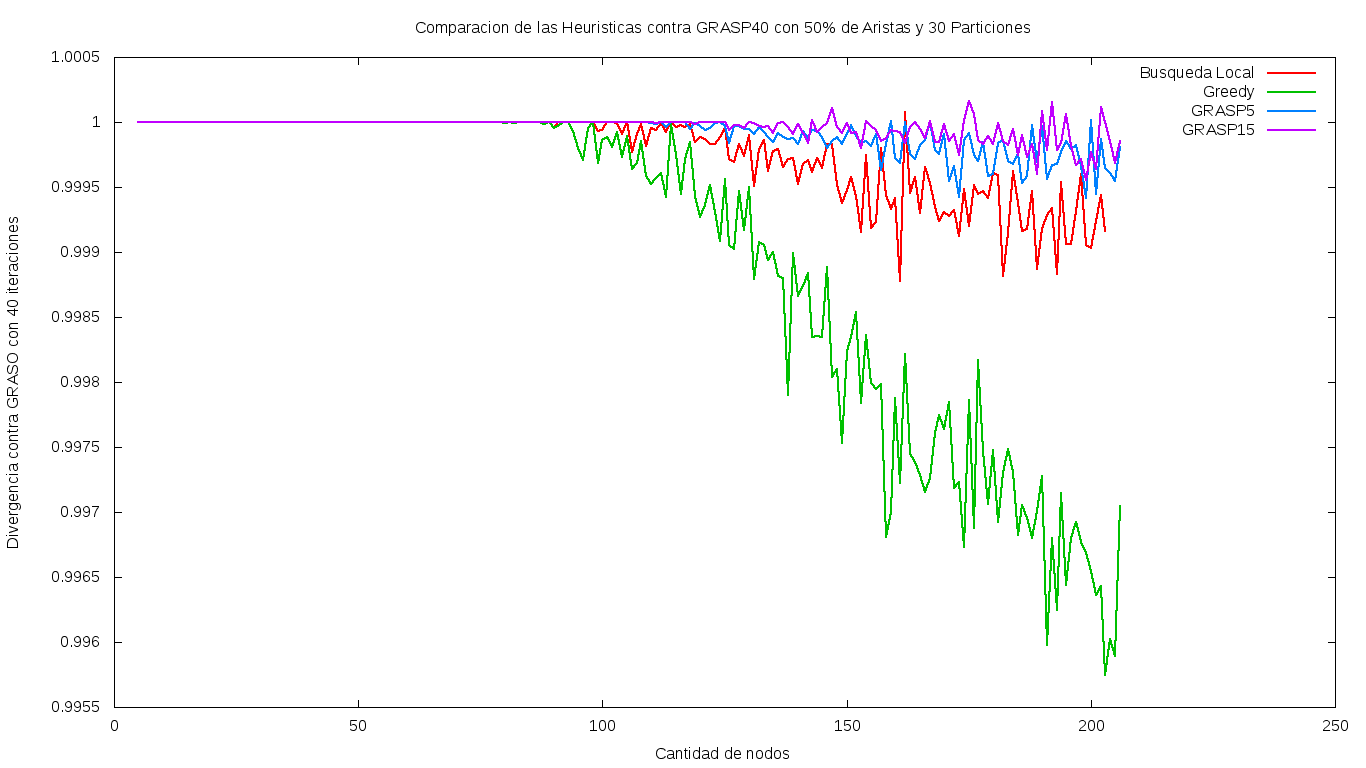
\includegraphics[scale=0.4]{finales/muchosComparacionesCon30Particiones50Aristas.png}
\caption{Distancias de las solucioens para K = 30 y 50\% de aristas}
\end{center}
\end{figure}

\begin{figure}[H]
\begin{center}
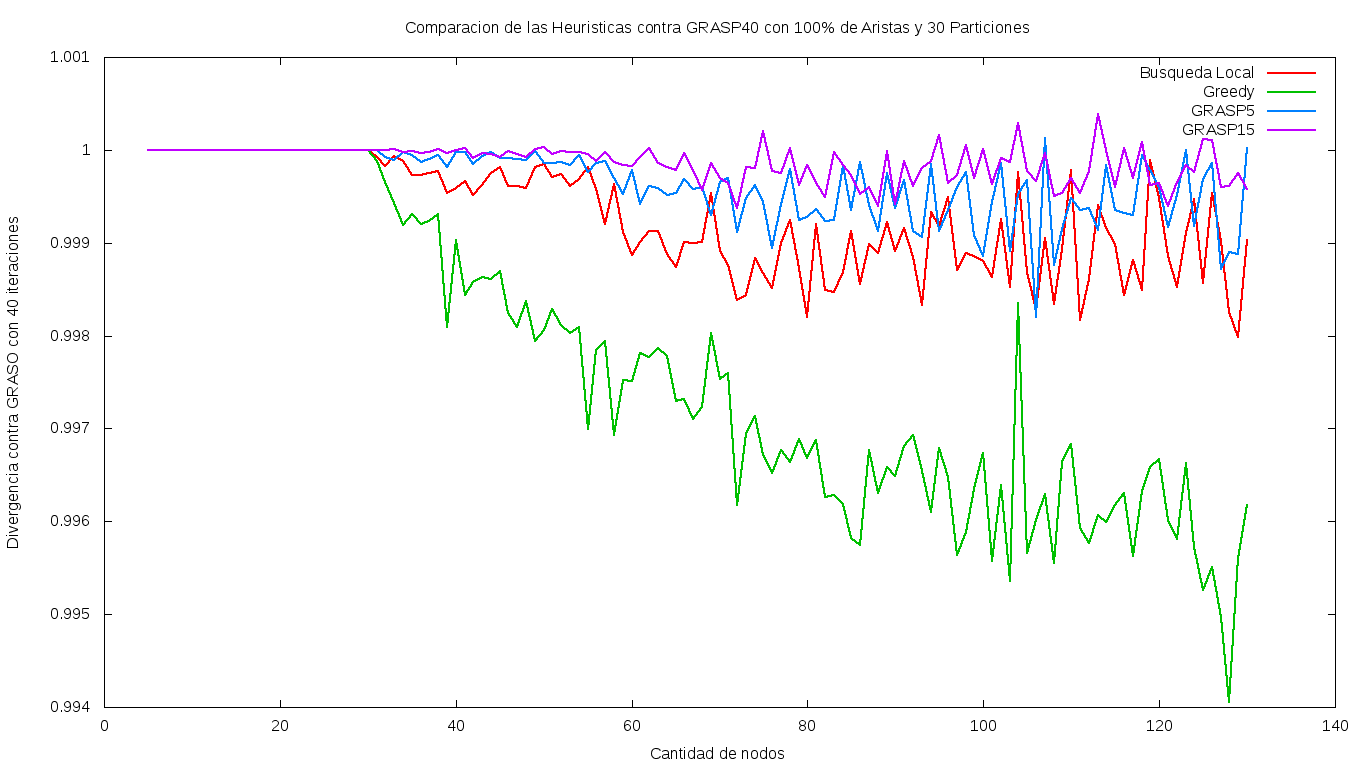
\includegraphics[scale=0.4]{finales/muchosComparacionesCon30Particiones100Aristas.png}
\caption{Distancias de las solucioens para K = 30 y 100\% de aristas}
\end{center}
\end{figure}

\subsubsection{70 Particiones}

\begin{figure}[H]
\begin{center}
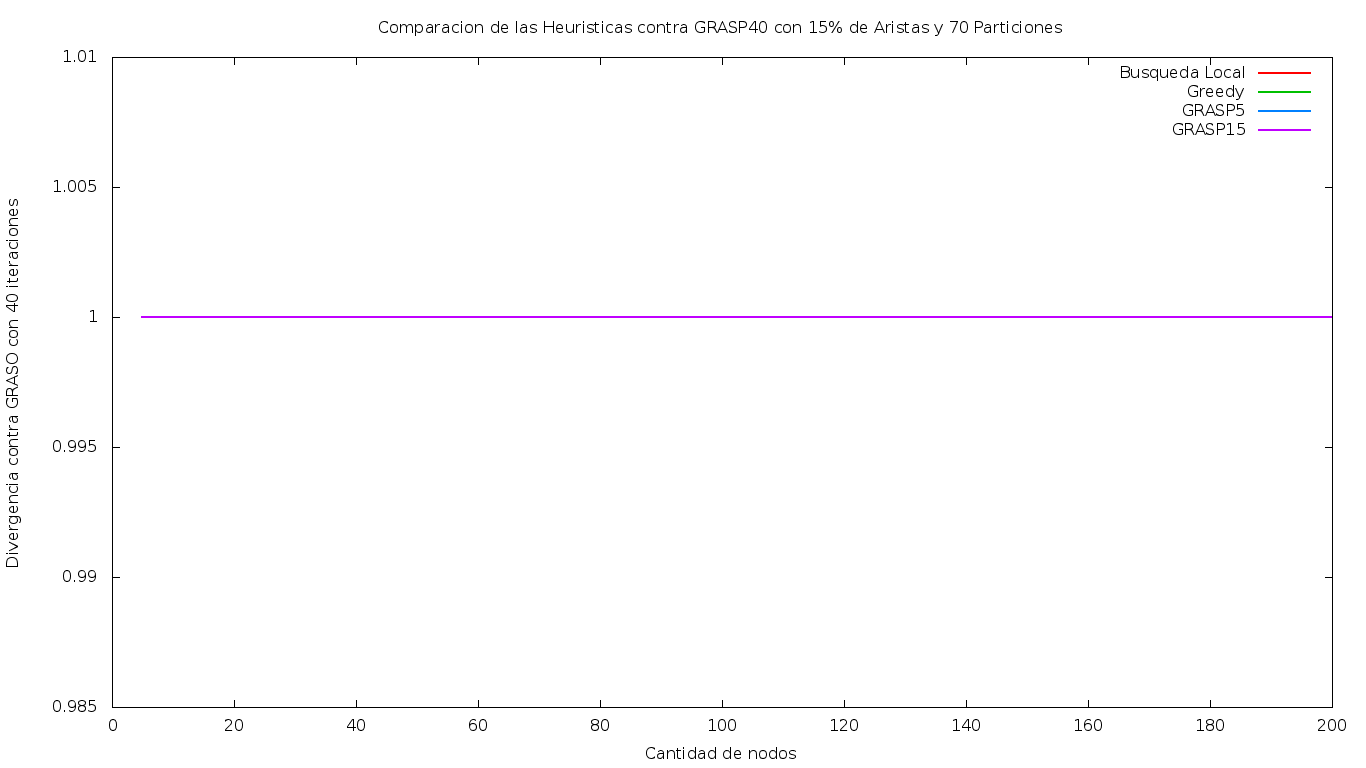
\includegraphics[scale=0.4]{finales/muchosComparacionesCon70Particiones15Aristas.png}
\caption{Distancias de las soluciones para K = 70 y 15\% de aristas}
\end{center}
\end{figure}

\begin{figure}[H]
\begin{center}
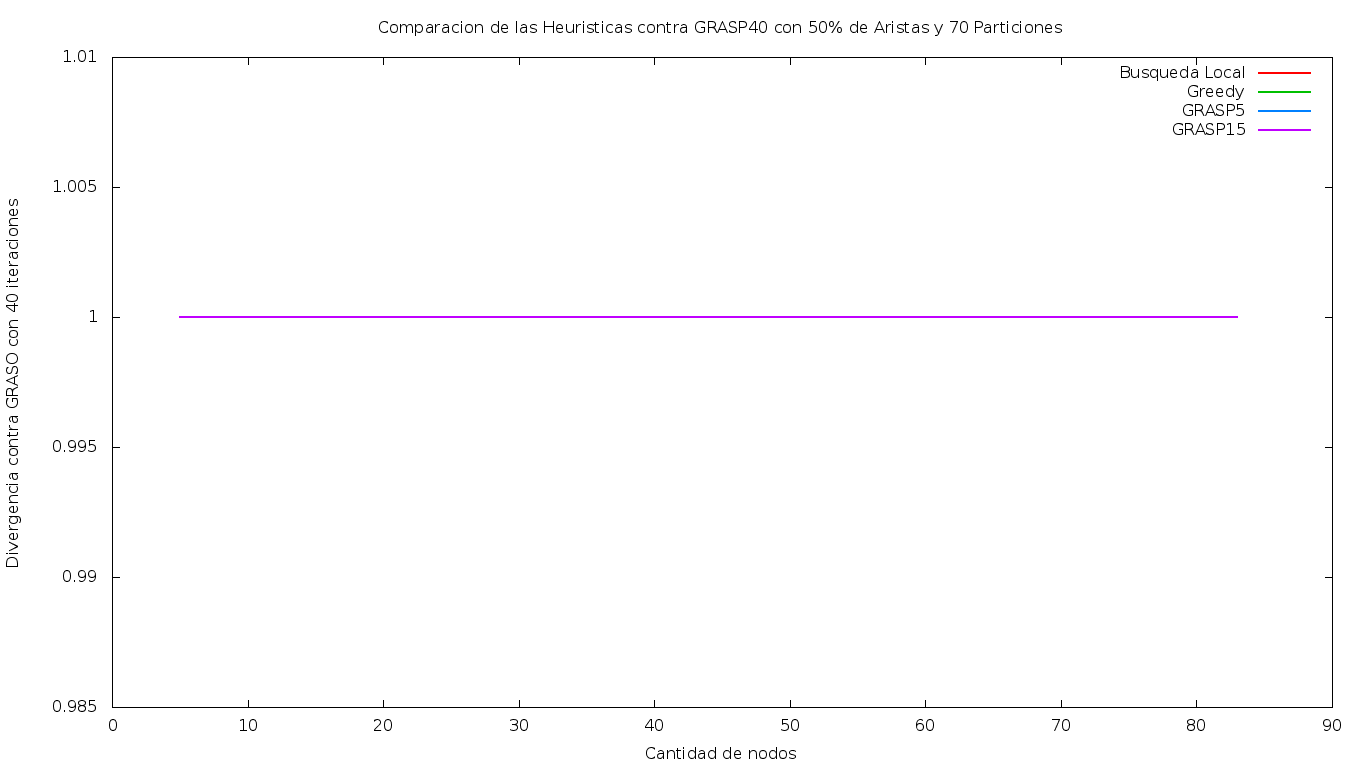
\includegraphics[scale=0.4]{finales/muchosComparacionesCon70Particiones50Aristas.png}
\caption{Distancias de las solucioens para K = 70 y 50\% de aristas}
\end{center}
\end{figure}

\begin{figure}[H]
\begin{center}
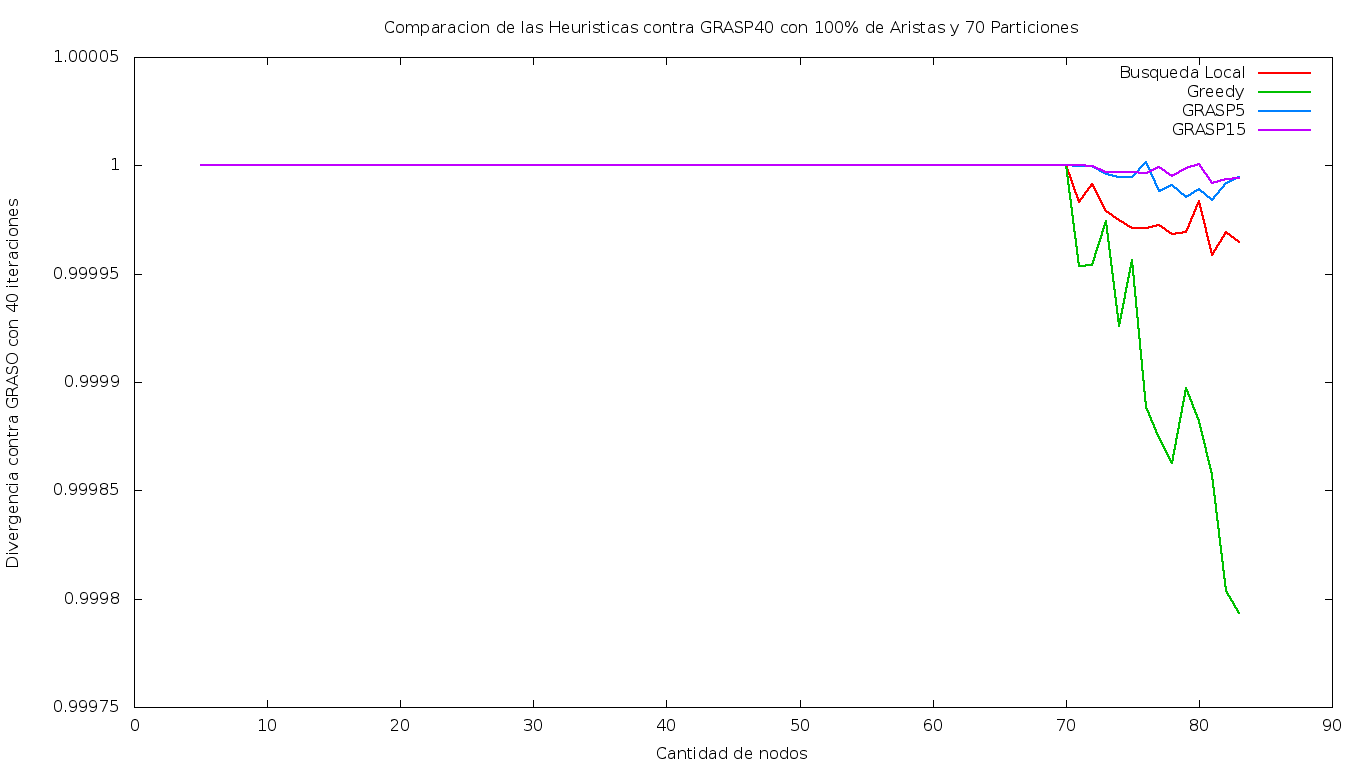
\includegraphics[scale=0.4]{finales/muchosComparacionesCon70Particiones100Aristas.png}
\caption{Distancias de las solucioens para K = 70 y 100\% de aristas}
\end{center}
\end{figure}


Luego de estos neuvos experimentos tenemos nuevas conclusiones pero tamb\'ien nuevas dudas.

Por ejemplo se puede corroborar claramente el orden de eficiencia de las Heuristicas, desde la peor siendo la Greedy, luego las Busqueda local, para finalizar con la GRASP con sus distinta cantidad de iteraciones (A mayor cantida de iteraciones, mayor calidad de la soluci\'on).\\

Luego tambien podemos corroborar como la cantidad de particiones y la densidad de los grafos marcan un corte desde el cual comienzan a incrementar las diferencias entre las soluciones de los distintos algoritmos. Por ejemplo vemo como para 30 particiones cuando la cantidad de nodos no supera los 30 todos los algoritmos retornan la soluci\'on optima que es la de peso 0. M\'as a\'un, para una densidad menor del grafo, con 30 particiones vemos como para el 50\% de las aristas siguen retornando todos la mejor soluci\'on (que en este caso no se puede afirmar que sea de peso 0) hasta casi instancias del problema con 90 nodos.

Luego de todo esto pudimos percibir ciertos comportamientos llamativos.

Por ejemplo hab\'iamos pensado que aumentando la cantidad de nodos y que la relaci\'on entre la cantida de particiones y cantidad de nodos, sea amplimente superada, iba a producir que la distancia de la soluci\'on de las Heuristicas se alejen cada vez m\'as de los valores \'optimos.

Pero por un lado podemos ver que para todos los algoritmos y sin importar la cantidad de nodos ni la relaci\'on entre las particiones y la cantidad de nodos, que la variaci\'on entre los mejores resultados y los peores es muy peque\'na. No llega a alejarse m\'as del 0.92 dentro de esta escala que fijamos para comparar resultados.\\

Lo m\'as llamativo es que todos los algoritmos parecieran a converger a un valor estable de distancia en relaci\'on a la mejor soluci\'on, como podemos ver en el gr\'afico para 5 particiones con el 100\% de las aristas.